

\section{Evaluating Multilingual Coherence}
\label{sec:eval}

A multilingual topic contains one topic for each
language.  For a multilingual topic to be meaningful to humans
(Figure~\ref{fig:example}), the meanings should be consistent across
the languages, in addition to coherent within each language
(\textit{i.e.}, all words in a topic are related).

This section describes our approach to evaluating the quality of
multilingual topics.  After defining the multilingual topic model, we
describe topic model evaluation extending standard monolingual
approaches to multilingual settings.

\subsection{Multilingual Topic Modeling}

Probabilistic topic models associate each document in a corpus with a
distribution over latent topics, while each topic is associated with a
distribution over words in the vocabulary.  The most widely used topic
model, latent Dirichlet allocation~\cite[\textsc{lda}]{blei2003}, can
be extended to connect languages.  These extensions require additional
knowledge to link languages together.

One common encoding of multilingual knowledge is \textbf{document
  links} (indicators that documents are parallel or comparable), used
in polylingual topic models~\cite{MimnoWNSM09,NiSHC09}.  In these
models, each document $d$ indexes a tuple of parallel/comparable
language-specific documents, $d^{(\ell)}$, and the language-specific
``views'' of a document share the document-topic distribution $\theta_d$.  The
generative story for the document-links model is: {
  \setlength{\interspacetitleruled}{0pt}
  \setlength{\algotitleheightrule}{0pt}
	\begin{algorithm}
	\small
	\For{each topic $k$ and each language $\ell$}{
		Draw a distribution over words $\phi_{\ell k} \sim \textrm{Dirichlet}(\beta)$\;
	}
	\For{each document tuple $d=\left(d^{(1)},\ldots,d^{(L)}\right)$}{
		Draw a distribution over topics $\theta_d \sim \textrm{Dirichlet}(\alpha)$\;
		\For{each language $\ell=1,\ldots,L$}{
			\For{each token $t\in d^{(\ell)}$}{
				Draw a topic $z_n\sim\theta_d$\;
				Draw a word $w_n\sim\phi_{\ell z}$\;
			}
		}

	}
	\end{algorithm}
}

Alternatively, word translations~\cite{JagarlamudiD10}, concept links~\cite{GutierrezSLMG16,YangBR17}, and multi-level
priors~\cite{KrstovskiSK16} can also provide multilingual
knowledges.  Since
the polylingual topic model is the most common approach for building
multilingual topic
models~\cite{VulicSM13,VulicSTM15,LiuDM15,KrstovskiS16}, our study
will focus on this model.







\subsection{Monolingual Evaluation}





Most automatic topic model evaluation metrics use co-occurrence
statistics of word pairs from a reference corpus to evaluate topic
coherence, assuming that coherent topics contain words that often
appear together~\cite{NewmanLGB10}.  The most
successful~\cite{LauNB14} is normalized pointwise
mutual information \cite[\npmi{}]{bouma}.  \npmi{} compares the joint
probability of words appearing together $\Pr(w_i,w_j)$ to their
probability assuming independence $\Pr(w_i)\Pr(w_j)$, normalized by
the joint probability:
\begin{align}
\label{eq:npmi}
\npmi{}(w_i, w_j) = \frac{\log \frac{\Pr(w_i,w_j)}{\Pr(w_i)\Pr(w_j)}}{\log\Pr(w_i,w_j)}.
\end{align}
The word probabilities are calculated from a {\bf reference corpus},
$\mathcal{R}$, typically a large corpus such as Wikipedia that can
provide meaningful co-occurrence patterns that are independent of the
target dataset.

The quality of topic $k$ is the average \npmi{} of
all word pairs $(w_i,w_j)$ in the topic:
\begin{align}
\hspace{-5pt}
\npmi{}_k = \frac{-1}{\binom{C}{2}}\sum_{i \in \mathcal{W}(k, C)} \sum_{j \neq i} \npmi{}(w_i, w_j),
\end{align}
where $\mathcal{W}(k, C)$ are the $C$ most probable words in
the topic-word distribution $\phi_k$ (the number of words is the
topic's \textbf{cardinality}).  Higher 
$\npmi{}_k$ means the topic's top words are more coupled.


\subsection{Existing Multilingual Evaluations}

While automatic evaluation has been well-studied for monolingual topic
models, there are no robust evaluations for multilingual topic models.
We first consider two straightforward metrics that could be used for
multilingual evaluation, both with limitations. We then propose an
extension of \npmi{} that addresses these limitations.

\paragraph{Internal Coherence.}

A simple adaptation of \npmi{} is to
calculate the monolingual \npmi{} score for each language
independently and take the average.  We refer this as internal \npmi{}
(\inpmi{}) as it evaluates coherence \textit{within} a language.
However, this metric does not consider whether the topic is coherent
\textit{across} languages---that is, whether a language-specific word
distribution $\phi_{\ell_1k}$ is related to the corresponding
distribution in another language, $\phi_{\ell_2k}$.

\paragraph{Crosslingual Consistency.}

Another straightforward measurement is Matching Translation
Accuracy~\cite[\mta{}]{Boyd-Graber:Blei-2009}, which counts the number
of word translations in a topic between two languages using a
bilingual dictionary.  This metric can measure whether a topic is
well-aligned across languages \textit{literally}, but cannot capture
non-literal more holistic similarities across languages.

\begin{figure}[t!]
	\centering
	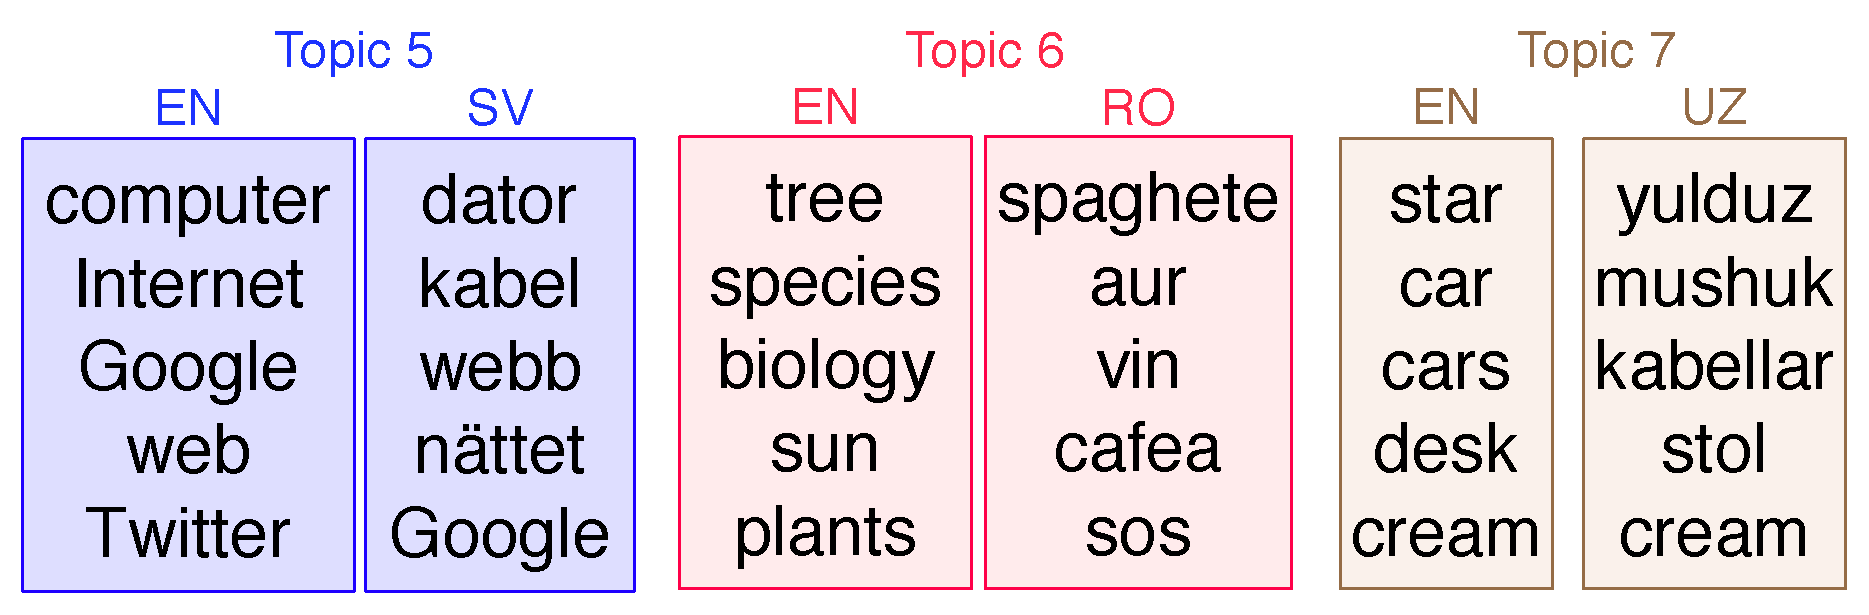
\includegraphics[width=\linewidth]{2018_naacl_mltm_eval/figures/topic_examples}
	\caption{Topic 5 is multilingually coherent: both the English and
		Swedish topics are about \underline{technology}. Topic 6 is about
		\underline{biology} in English but \underline{food} in Romanian, so
		it is low quality although coherent monolingually. Topic 7
		is monolingually incoherent, so it is a low quality topic even if
		it contains word translations.}
	\label{fig:example}
\end{figure}


\subsection{New Metric: Crosslingual \npmi}

We extend \npmi{} to multilingual models, with a metric we
call crosslingual normalized pointwise mutual information (\cnpmi{}).
This metric will be the focus of our experiments.

A multilingually coherent topic means that if $w_{i,\ell_1}$ in language $\ell_1$
and $w_{j,\ell_2}$ in language $\ell_2$ are in the same topic, they should appear
in similar contexts in comparable or parallel corpora
$\mathcal{R}^{(\ell_1,\ell_2)}$.
Our adaptation of \npmi{} is based on the
same principles as the monolingual version,
but focuses on the
co-occurrences of \textit{bilingual} word pairs.
Given a bilingual word pair $\left(w_{i,\ell_1},w_{j,\ell_2}\right)$
the co-occurrence of this word pair is the event
where word $w_{i,\ell_1}$ appears in a document in language~$\ell_1$
and the word $w_{j,\ell_2}$ appears in a comparable or parallel document in language~$\ell_2$.


The co-occurrence probability of each bilingual word pair is:
	\begin{align}
	\begin{split}
		&\Pr\left(w_{i,\ell_1},w_{j,\ell_2}\right) \\ & \triangleq  \frac{\left|\left\lbrace{\mathbf{d}}: w_{i,\ell_1}\in{d}^{(\ell_1)},w_{j,\ell_2}\in{d}^{(\ell_2)}\right\rbrace\right|}{\left|\mathcal{R}^{(\ell_1,\ell_2)}\right|},
	\end{split}
	\end{align}
where $\mathbf{d}=\left(d^{(\ell_1)}, d^{(\ell_2)}\right)$ is
a pair of parallel/comparable documents in the
reference corpus $\mathcal{R}^{(\ell_1,\ell_2)}$. 
When one or both words in a bilingual pair do not appear in the reference
corpus, the co-occurrence score is zero.











        
        
        
        
	
	
	


Similar to monolingual settings,
\cnpmi{}
for a bilingual topic $k$ is the average of the
\npmi{} scores of all $C^2$ bilingual word pairs,
\begin{align}\hspace{-8.5pt}
\cnpmi{}(\ell_1,\ell_2,k) = \frac{\sum_{i,j}^{C}\npmi{}\left(w_{i,\ell_1},w_{j,\ell_2}\right)}{C^2}.
\end{align}
It is straightforward to generalize \cnpmi{} from a language pair to multiple
languages by averaging \cnpmi$(\ell_i,\ell_j,k)$ over all language
pairs $(\ell_i,\ell_j)$.